\documentclass[journal]{IEEEtran}
\usepackage[a5paper, margin=10mm, onecolumn]{geometry}
\usepackage{lmodern}
\usepackage{tfrupee}
\setlength{\headheight}{1cm}
\setlength{\headsep}{0mm}

\usepackage{gvv-book}
\usepackage{gvv}
\usepackage{cite}
\usepackage{amsmath,amssymb,amsfonts,amsthm}
\usepackage{algorithmic}
\usepackage{graphicx}
\usepackage{textcomp}
\usepackage{xcolor}
\usepackage{txfonts}
\usepackage{listings}
\usepackage{enumitem}
\usepackage{mathtools}
\usepackage{gensymb}
\usepackage{comment}
\usepackage[breaklinks=true]{hyperref}
\usepackage{tkz-euclide}
\usepackage{listings}
\def\inputGnumericTable{}
\usepackage[latin1]{inputenc}
\usepackage{color}
\usepackage{array}
\usepackage{longtable}
\usepackage{calc}
\usepackage{multirow}
\usepackage{hhline}
\usepackage{ifthen}
\usepackage{lscape}
\usepackage{xparse}

\bibliographystyle{IEEEtran}

\title{4.11.20}
\author{EE25BTECH11043 - Nishid Khandagre}
\begin{document}
\maketitle

\renewcommand{\thefigure}{\theenumi}
\renewcommand{\thetable}{\theenumi}

\numberwithin{equation}{enumi}
\numberwithin{figure}{enumi}

Question:
Find the coordinates of the point where the line through the points $\vec{A} \myvec{3\\4\\1}$ and $\vec{B}\myvec{5\\1\\6}$ crosses the $XZ$ plane. Also find the angle which this line makes with the $XZ$ plane.

Solution: 
Direction vector
\begin{align}
    \vec{d} &= \vec{B} - \vec{A}\\
    &=\myvec{5 \\ 1 \\ 6} - \myvec{3 \\ 4 \\ 1} = \myvec{2 \\ -3 \\ 5}
\end{align}
The normal vector $\vec{n}$ to the $XZ$-plane is:
\begin{align}
    \vec{n} = \myvec{0 \\ 1 \\ 0}
\end{align}
General point $\vec{P}$ on the line
\begin{align}
    \vec{P} = \vec{A} + t\vec{d}
\end{align}

For the line to intersect the $XZ$-plane, the point $\vec{P}$ must lie on the plane.
Therefore
\begin{align}
    \vec{n}^\top\vec{P}&=0\\
    \vec{n}^\top (\vec{A} + t\vec{d}) &= 0 \\
    \vec{n}^\top \vec{A} + t \, \vec{n}^\top \vec{d} &= 0 \\
    t &= -\frac{\vec{n}^\top \vec{A}}{\vec{n}^\top \vec{d}}
\end{align}

\begin{align}
    \vec{n}^\top \vec{A} &= \myvec{0 & 1 & 0} \myvec{3 \\ 4 \\ 1} = 4 \\
    \vec{n}^\top \vec{d} &= \myvec{0 & 1 & 0} \myvec{2 \\ -3 \\ 5} = -3
\end{align}

\begin{align}
    t = -\frac{4}{-3} = \frac{4}{3}
\end{align}
Intersection point:
\begin{align}
\vec{P} &= \vec{A} + \frac{4}{3}\vec{d}\\
&=\myvec{3 \\ 4 \\ 1} + \frac{4}{3}\myvec{2 \\ -3 \\ 5}\\
&=\myvec{\frac{17}{3} \\ 0 \\ \frac{23}{3}}
\end{align}
The angle $\theta$ between a line with direction vector $\vec{d}$ and a plane with normal vector $\vec{n}$ is given by:
\begin{align}
\sin\theta &= \frac{|\vec{n}^\top \vec{d}|}{\norm{\vec{n}}\norm{\vec{d}}}
\end{align}
\begin{align}
\norm{\vec{n}}=\sqrt{\vec{n}^\top\vec{n}}
\end{align}
\begin{align}
\norm{\vec{n}}&=\sqrt{0^2 + 1^2 + 0^2}\\
\norm{\vec{n}}&= 1
\end{align}
\begin{align}
\norm{\vec{d}}=\sqrt{\vec{d}^\top\vec{d}}
\end{align}
\begin{align}
\norm{\vec{d}}&= \sqrt{2^2 + (-3)^2 + 5^2}\\
\norm{\vec{d}}&=\sqrt{38}
\end{align}
\begin{align}
    \sin\theta &= \frac{|-3|}{1 \cdot \sqrt{38}} = \frac{3}{\sqrt{38}}
\end{align}


\begin{figure}[H]
\centering
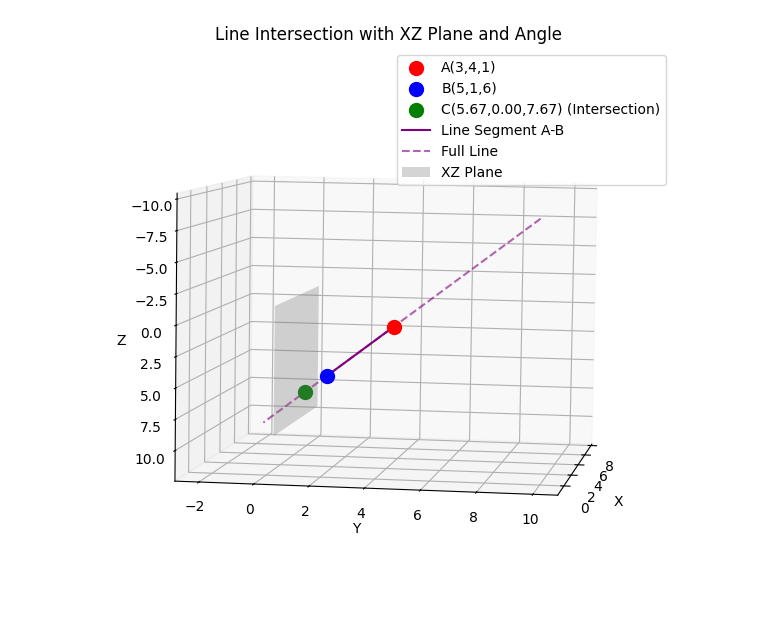
\includegraphics[width=0.8\columnwidth]{figs/fig1.png}
\caption{}
\label{fig:1}
\end{figure}

\end{document}
